\documentclass[12pt]{article}
%\documentclass{article}

\usepackage{times}
\usepackage[final]{graphicx}
\usepackage{hyperref}

\setlength{\topmargin}{-0.5in}
\setlength{\oddsidemargin}{0in}
\setlength{\evensidemargin}{0in}
\setlength{\textwidth}{6.5in}
\setlength{\textheight}{9.0in}

\begin{document}

\centerline{\bf \Large CS295/CS395/CSYS395: \href{CS295_395_Syllabus.pdf}{\underline{Evolutionary Robotics}}}

\vspace{0.5cm}

\centerline{\bf \large Programming Assignment 2 of 10}

\vspace{0.5cm}

\centerline{\large Assigned: Friday, September 9, 2011}

\vspace{0.5cm}

\centerline{\large Due: Friday, September 16, 2011 by midnight}

\vspace{0.5cm}

\noindent \textbf{Description:} In this assignment you will be creating an \href{http://en.wikipedia.org/wiki/Artificial_neural_network}{\underline{artificial neural network}} (ANN). There are many kinds of ANNs, but they all share one thing in common: they are represented as a directed graph in which the nodes are models of biological neurons, and edges are models of biological synapses. Henceforth, the terms `neurons' and `synapses' will be used to describe the elements of an ANN. The behavior, in addition to the structure of an ANN is also similar to biological neural networks:
(1) each neuron holds a value which indicates its level of activation;
(2) each directed edge (synapse) is assigned a value, known as its `strength', which indicates how much influence the source neuron has on the target neuron; and
(3)  the activation $a$ of a neuron $i$ at the next time step is usually expressed as
\begin{eqnarray}
a_i = \sigma ( \sum_{j=1}^{n} w_{ij}a_j )
\end{eqnarray}
where there are $n$ neurons that connect to neuron $i$,
$a_j$ is the activation of the $j$th neuron that connects to neuron $i$,
$w_{ij}$ is the weight of the synapse connecting neuron $j$ to neuron $i$,
and $\sigma()$ is a function that keeps the activation of neuron $i$ from growing too large.

In this project you will create an artificial neural network in Python, simulate its behavior over time, and visualize the resulting behavior. \\

\noindent \textbf{Tasks:}

\begin{enumerate}

\item \textbf{Back up your Python code from assignment 1.} Encapsulate your code from assignment 1 in a single file, Assignment\_1.py, such that when you run it you can reproduce all of the visualizations. This will prove to you that that code is working fine, as you will use it in this and subsequent assignments.

\item Make a copy of Assignment\_1.py and call it Assignment\_2.py. You will use the matrix functions you developed in assignment 1. 

\item First, we will create a neural network with 10 neurons. To do this, create a $50 \times 10$ matrix: element $e_{ij}$ will store the value of neuron $j$ at time step $i$. Name this matrix \textbf{\texttt{neuronValues}}.

\item Set each elements in the first row to a random value in $[0,1]$: these values will represent the initial values of the neurons.

\item To visualize the network, we will place the 10 neurons in a circular pattern as shown in Fig. \ref{Fig}a. Create a new matrix \textbf{\texttt{neuronPositions=MatrixCreate(2,10)}} which will store the two-dimensional position of each neuron such that \textbf{\texttt{neuronPositions[0,i]}} will store the x-value for neuron $i$ and \textbf{\texttt{neuronPositions[1,i]}} will store the y-value for neuron $i$.

\item Now, compute the positions of the neurons as follows:\\
\textbf{\texttt{angle = 0.0}}\\
\textbf{\texttt{angleUpdate = 2 * pi /numNeurons}}\\
\textbf{\texttt{for i in range(0,numNeurons)}}\\
\indent \textbf{\texttt{\hspace{1cm}x = sin(angle)}}\\
\indent \textbf{\texttt{\hspace{1cm}y = cos(angle)}}\\
\indent \textbf{\texttt{\hspace{1cm}angle = angle + angleUpdate}}\\

\item Now, use this matrix and the plot() function to create the visualization shown in Fig. \ref{Fig}a. Hint: to create circles, you need to use \textbf{\texttt{plot(...,'ko',markerfacecolor=[1,1,1]}}, \textbf{\texttt{markersize=18)}}. Copy and paste this visualization into your document.

\item To create the synapses, create a $10 \times 10$ matrix \textbf{\texttt{synapses}} and set each element to a value in $[-1,1]$. A synapse with a negative weight \textit{inhibits} its target neuron: the stronger the activation of the originating neuron, the lower the activation of the target neuron.

\item Create a plotting function that takes as input \textbf{\texttt{neuronPositions}} and draws a line between each pair of neurons. The resulting visualization should look like Fig. \ref{Fig}b. Store the resulting visualization in your document. \textbf{Note:} If you want to draw a line between the two points (x1,y1) and (x2,y2), you can use \textbf{\texttt{plot([x1,x2],[y1,y2])}}, and \underline{not} \textbf{\texttt{plot([x1,y1],[x2,y2])}}.

\item Modify your plotting function such that it takes as input \textbf{\texttt{neuronPositions}} and \textbf{\texttt{synapses}}, and draws gray lines
    (plot(...,color[0.8,0.8,0.8]))
    for negatively-weighted synapses and black lines
    (plot(...,color[0,0,0])) for positively-weighted synapses. Store the resulting visualization, which should look like Fig. \ref{Fig}c, in your document.

\item Modify your plotting function again such that the width of each line indicates the magnitude of the corresponding synapse's weight. \textbf{Note:} The width of a line must be an integer value: e.g., plot(...,linewidth=2). To convert a synaptic weight to a number in 1,2,... use w = int(10*abs(synapses[i,j]))+1, and then plot(...,linewidth=w). Store the resulting visualization, which should look like Fig. \ref{Fig}d, in your document.

\item Now create a function that updates each neuron in the network: \textbf{\texttt{neuronValues = Update}} (\textbf{\texttt{neuronValues,synapses,i)}}.
    (You created \textbf{\texttt{neuronValues}} in step 3.)
    This function will iterate through each element in the $i$th row of \textbf{\texttt{neuronValues}}, and compute the sum
    \begin{eqnarray}
    temp = \sum_{j=1}^{10} w_{ij} a_{j}
    \end{eqnarray}
    where $a_{j}$ is the value of the $j$th neuron on the previous row, and
    $w_{ij}$ is element $e_{ij}$ in the matrix \textbf{\texttt{synapses}}. If this temporary sum is less than zero, round it to zero; if it is larger than one, round it to one. Store the result in \textbf{\texttt{neuronValues}}. \textbf{Note:} Before updating the neurons, make sure to set each neuron to a random value in [0,1]. \textbf{Thing to think about:} If the neurons are all set to zero initially, what do you think their values will be in subsequent time steps?

\item Now use the matrix imaging function you developed in the previous assignment to visualize how the neuron values change over time. This should produce an image similar to that shown in Fig. \ref{Fig}e. Copy and paste the image into your document. The image does not need to look exactly like that of Fig. \ref{Fig}e. In fact, re-run your program several times, and compare the images produced. Notice that the patterns of neuron activation vary greatly from one run to the next. We will discuss why this is the case in class.

\item \textbf{Things to think about:} Why do some of the neurons oscillate like this? What happens when all of the synaptic weights are set to $-1$, or to zero, or to $1$? You do not need to include your answers in the document you submit for grading.

\end{enumerate}

\begin{figure}[!t]
\centerline{
a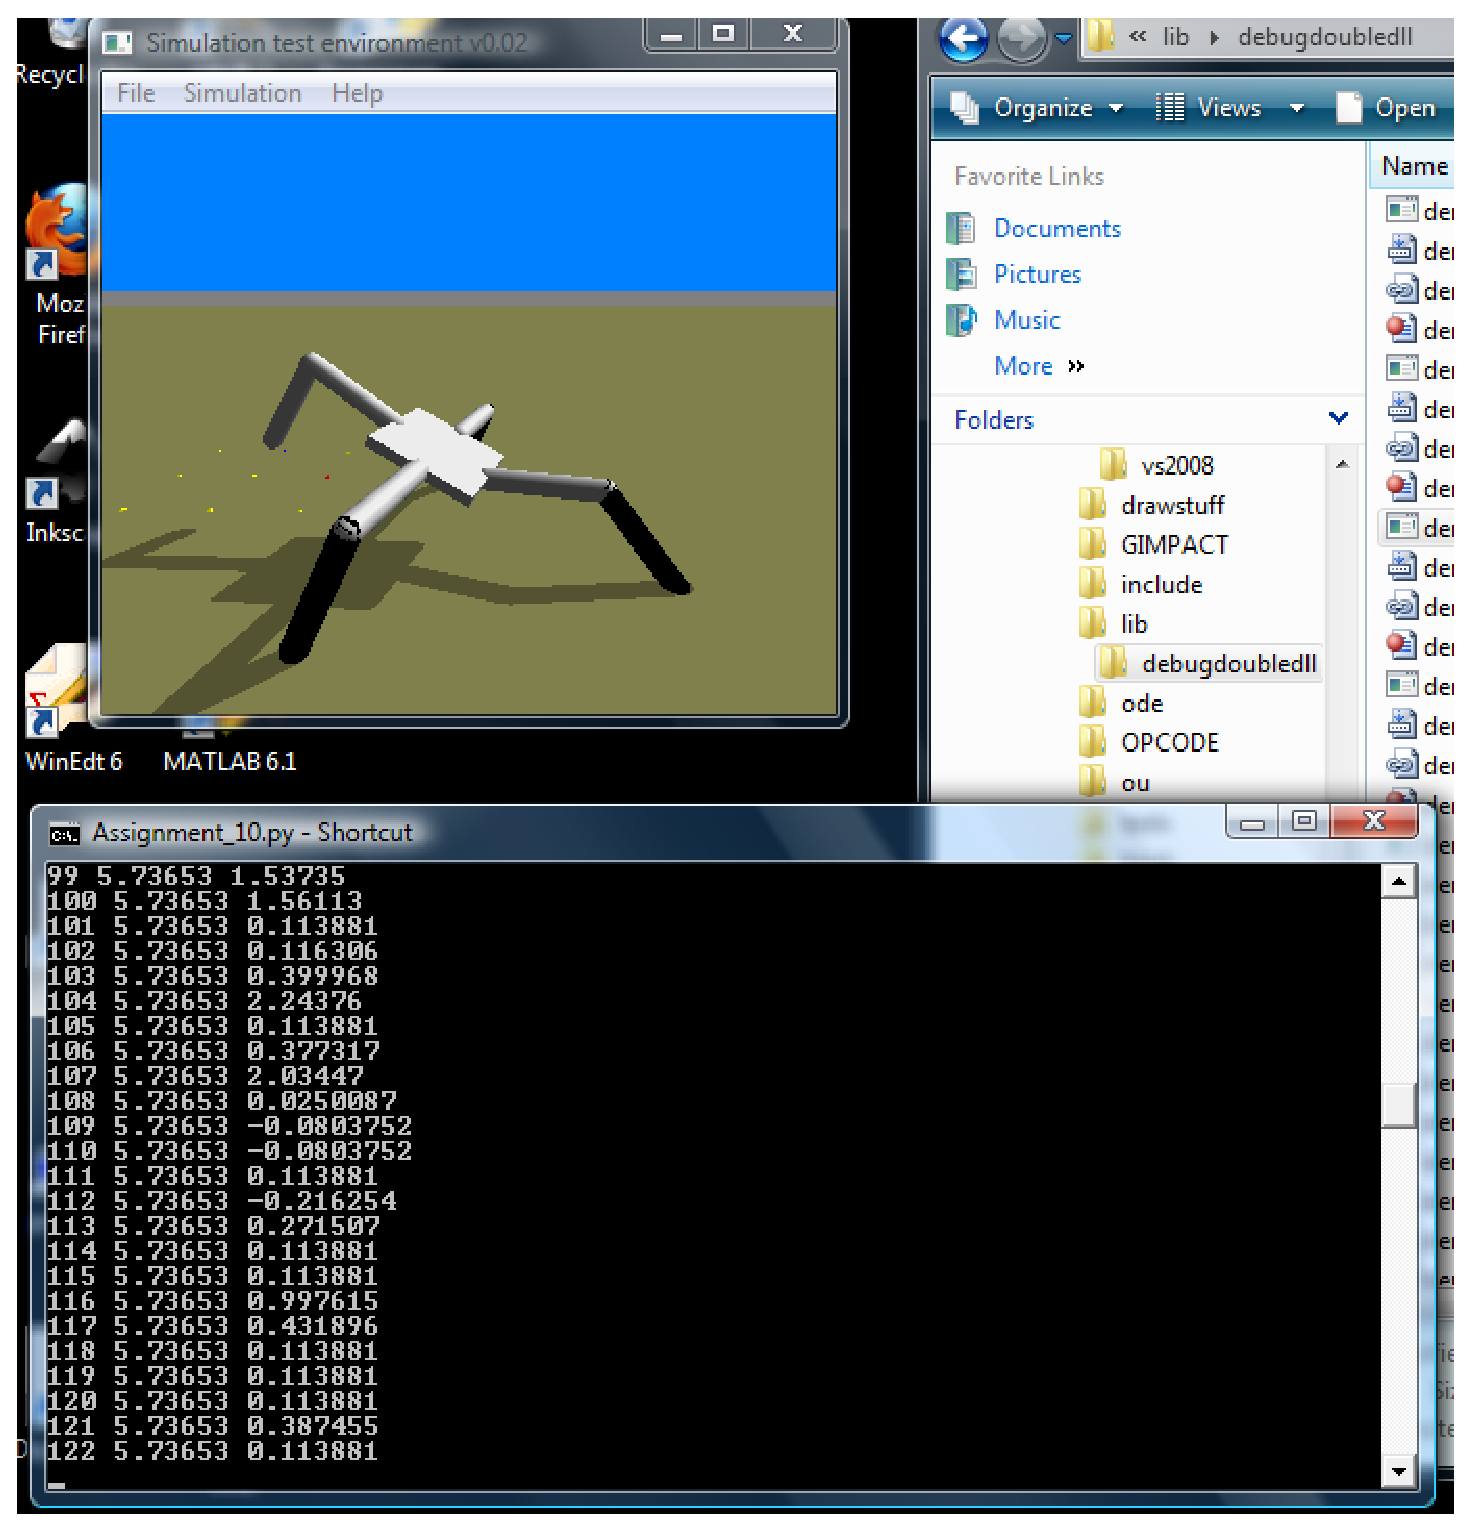
\includegraphics[width=0.45\textwidth]{Fig1}
b\includegraphics[width=0.45\textwidth]{Fig2}
}
\centerline{
c\includegraphics[width=0.45\textwidth]{Fig3}
d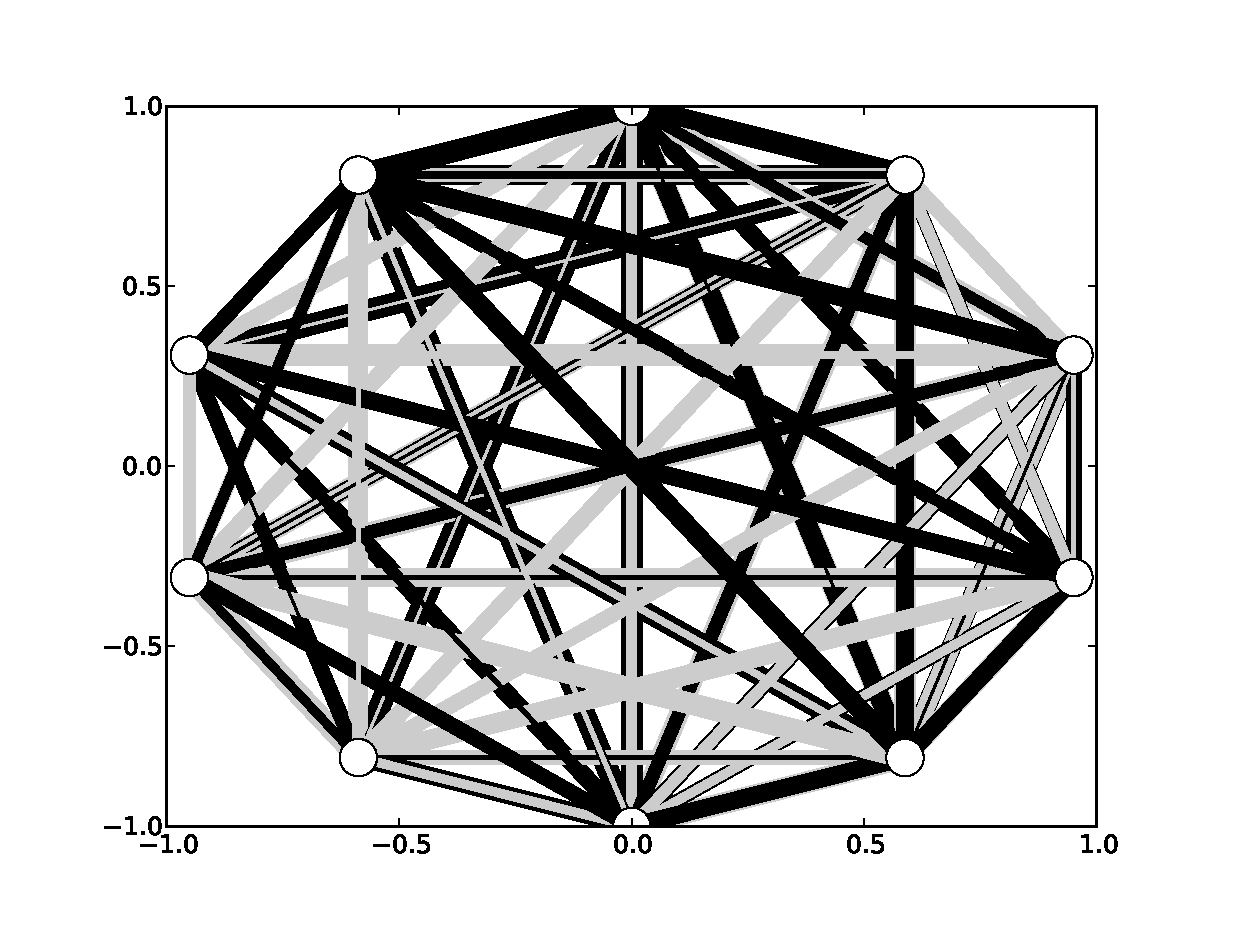
\includegraphics[width=0.45\textwidth]{Fig4}
}
\centerline{
e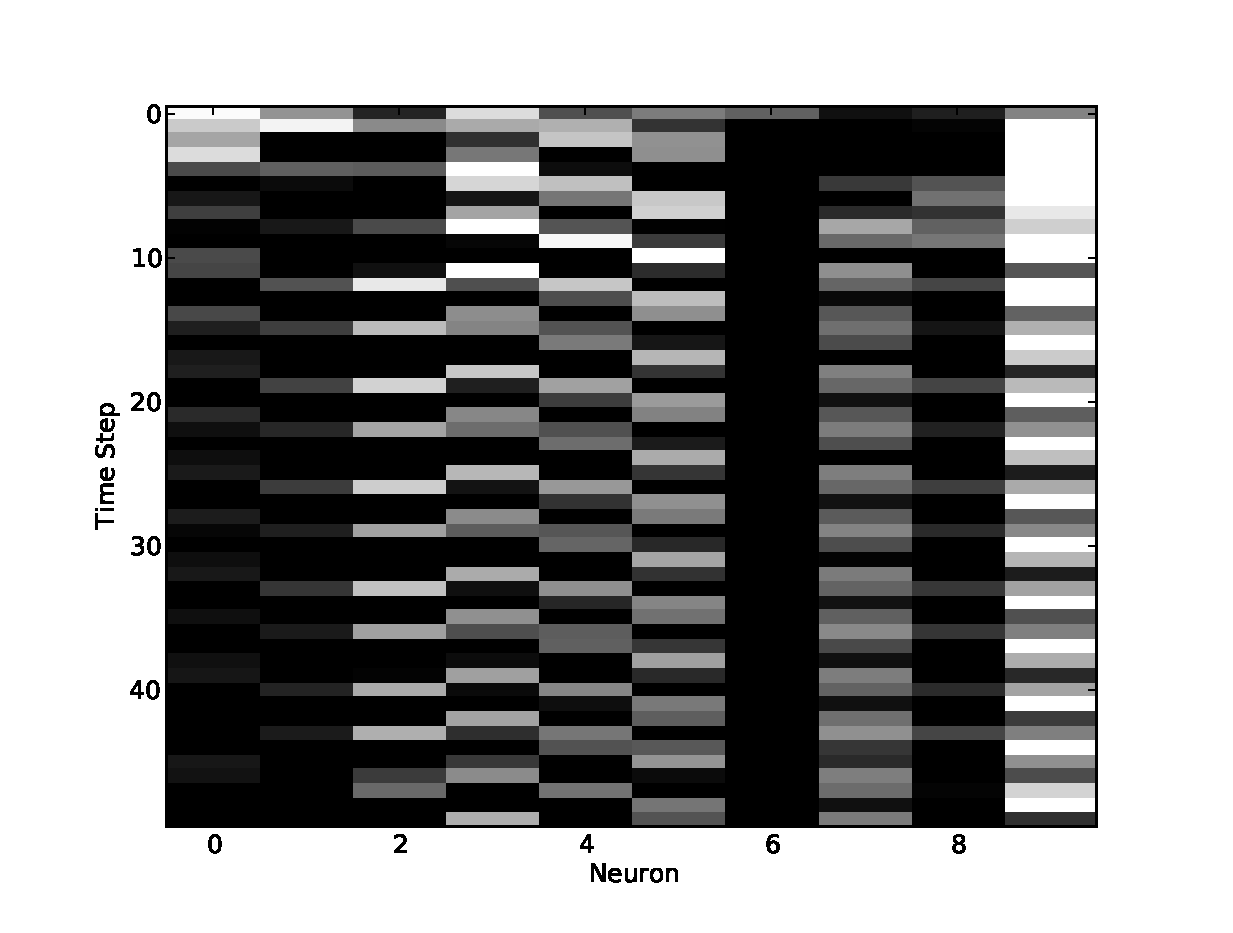
\includegraphics[width=0.45\textwidth]{Fig5}
}
\caption{Visualizations demonstrating the successful creation of an artificial neural network.
a: An ANN with 10 neurons and no synapses.
b: An ANN with 10 neurons and $10 \times 10 = 100$ synapses.
c: Gray and black lines indicate synapses with negative and positive weight, respectively.
d: Line width indicates the magnitude of the synapse's weight.
e: The pattern of neuron activity as time passes.}
\label{Fig}
\end{figure}

\end{document} 
